\input{../../Plantillas-Fomato/Tareas/tarea.tex}
\cabe{Geometría \textsc{iii}: Tarea 1}{Jhonny Lanzuisi, 1510759}

\begin{document}
		\thispagestyle{plain}
		\tituloD{Geometría 3}{Primera Tarea}
		\subsection*{Ejercicio 1}
		¿Qué figuras limitan las bisectrices de los ángulos de un paralelogramo (no rombo)?
	\begin{sol}
		 Consideremos el paralelogramo $ABCD$ y su centro de simetría $O$. Sean $\alpha,\beta,\gamma,\delta$ los ángulos en $A,B,C,D$ respectivamente, además, sean $r,s,t,u$ las bisectrices de los ángulos $\alpha,\beta,\gamma,\delta$ respectivamente. Los ángulos $\alpha,\gamma$ son homólogos por la simetría en $O$ y sus bisectrices también. Luego las bisectrices $r$ y $t$ son paralelas. Lo mismo ocurre para las bisectrices $s$ y $u$. De esto se sigue que la figura determinada por ellas es un paralelogramo.
		
		Más aún, este paralelogramo es rectángulo. Para ver esto, sea $E$ la intersección de las bisectrices $r$ y $s$ y consideremos el triángulo $\triangle ABE$. En este triángulo los ángulos en $A,B$ ($\alpha',\beta'$  respectivamente) han de sumar un ángulo recto puesto que son la mitad de la suma $\alpha+\beta=\pi$. Como los ángulos internos del triángulo han de sumar un ángulo llano se sigue que el ángulo en $E$ es recto. Este es opuesto por el vertice al ángulo $\angle GEF$ del paralelogramo delimitado por las bisectrices, por lo cual es un rectángulo.
		\begin{figure}[H]\centering
			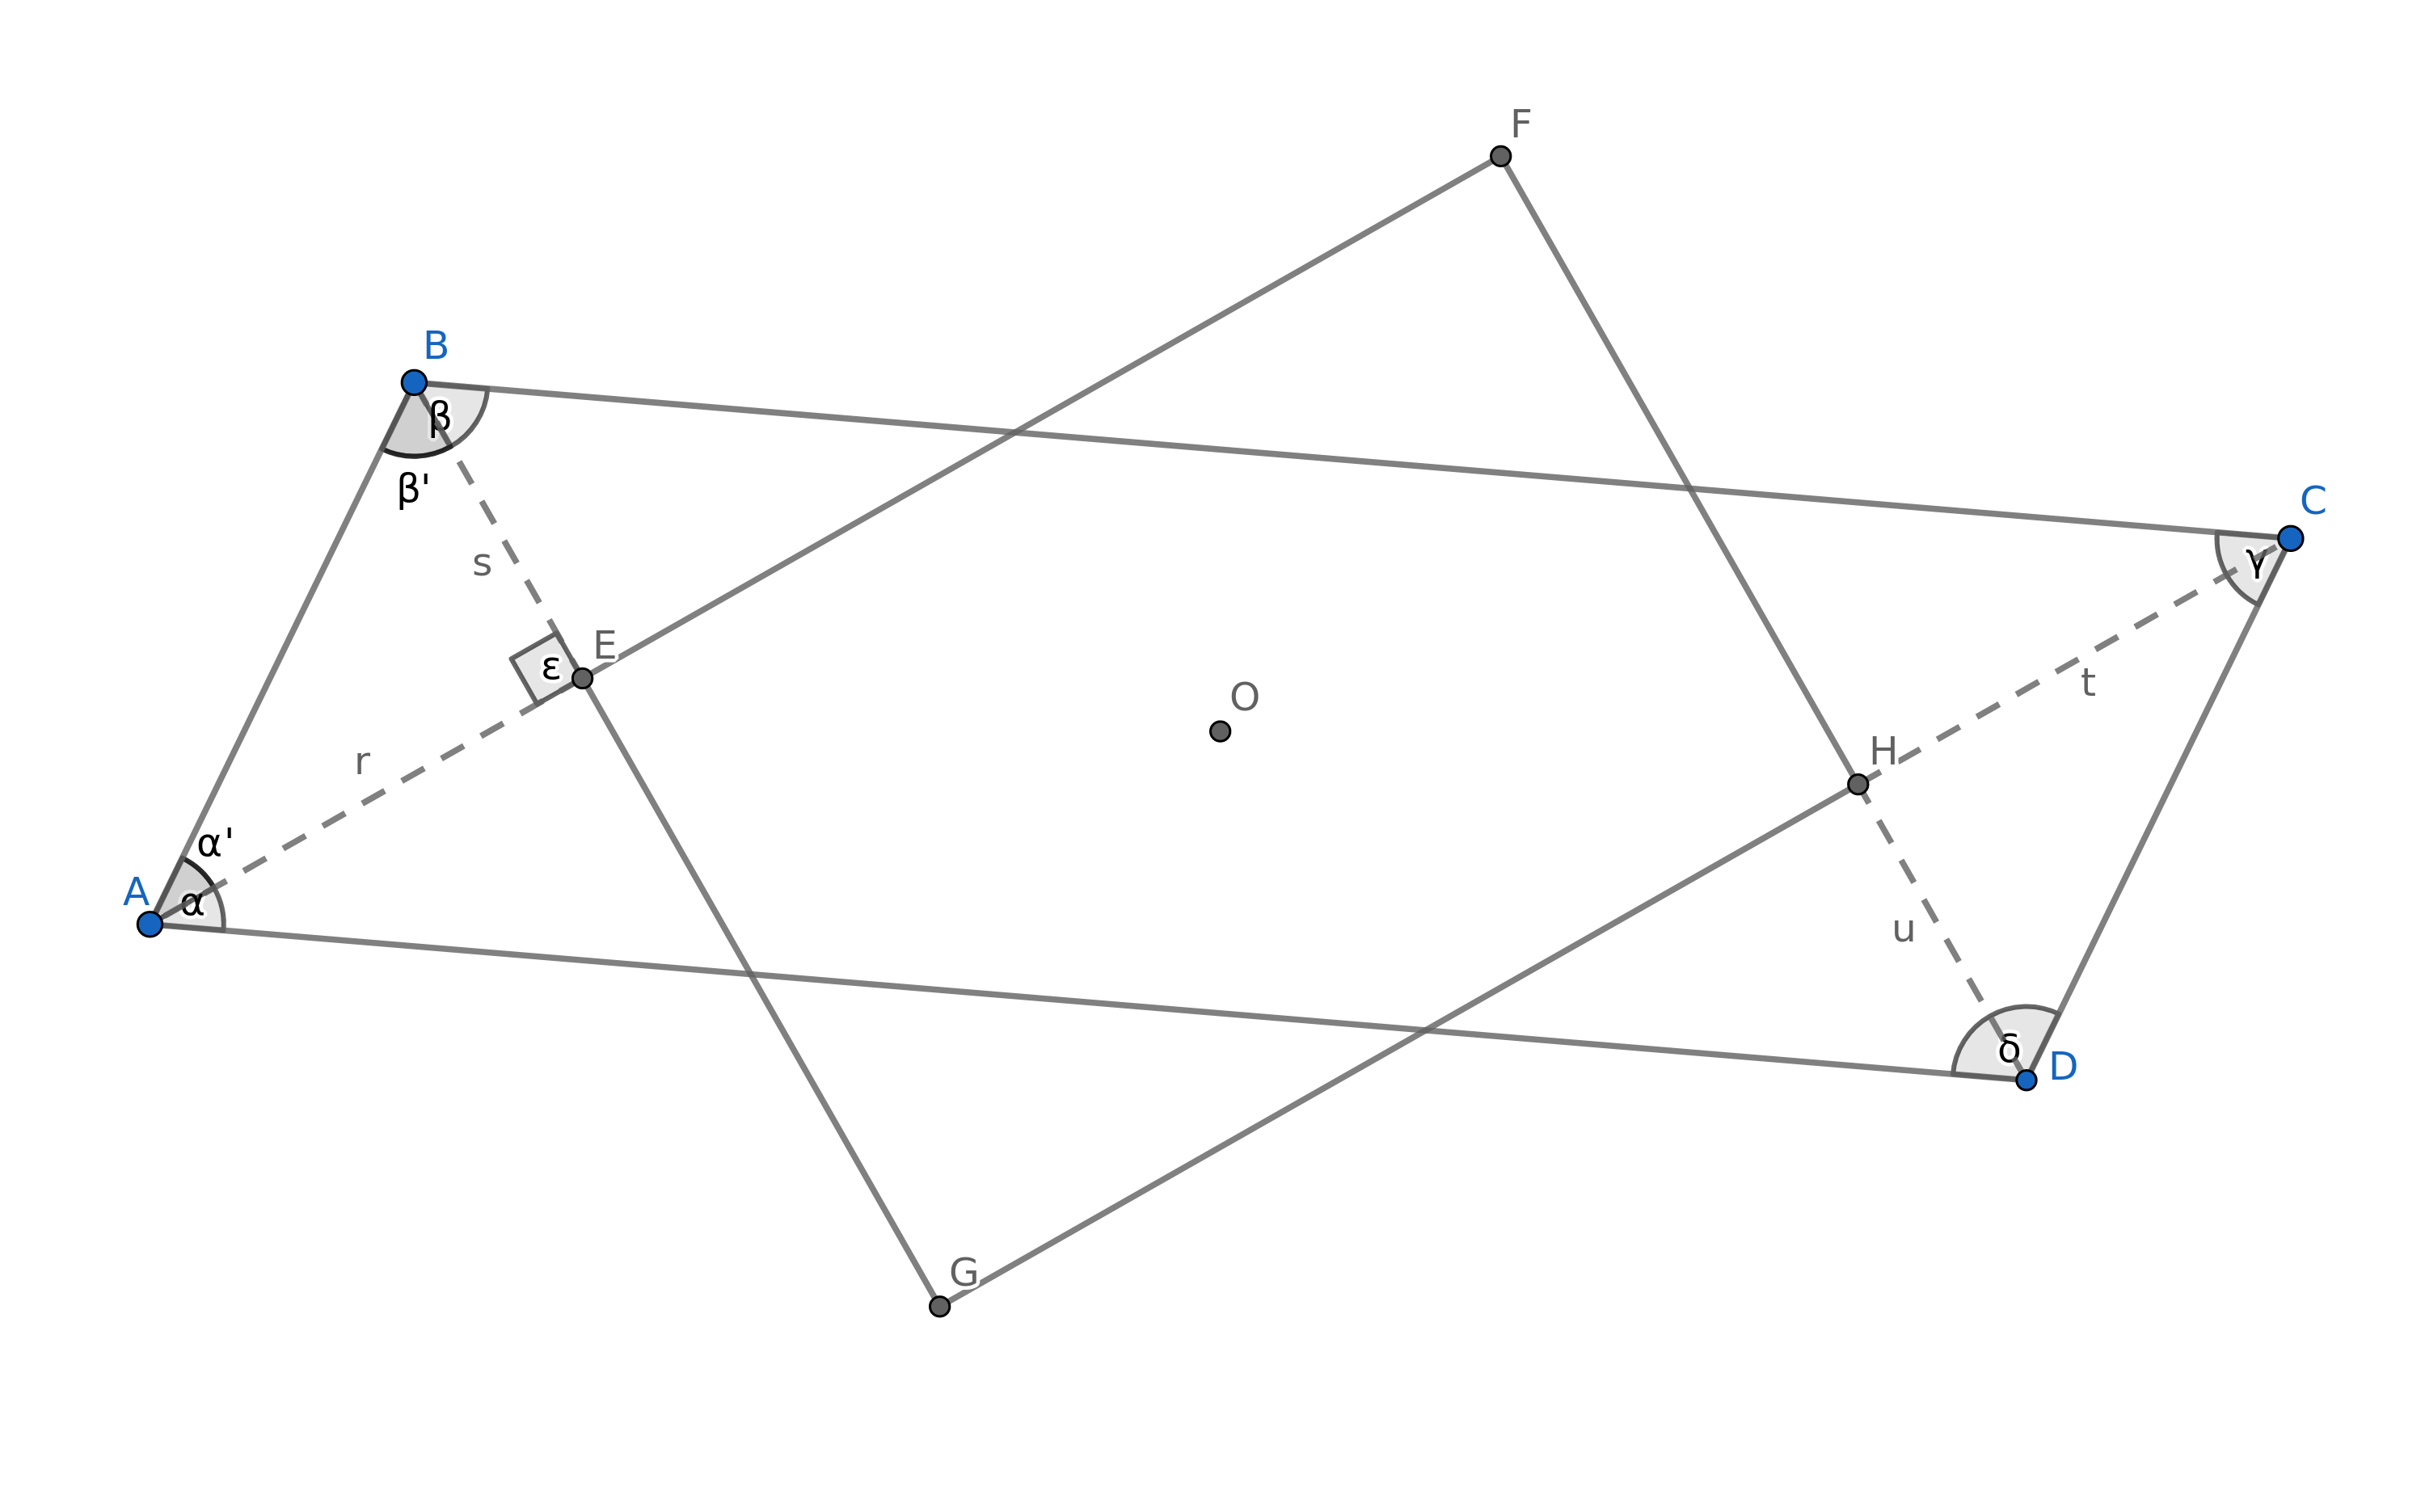
\includegraphics[width=1\linewidth]{pics/g1}
		\end{figure}
	\end{sol}

\subsection*{Ejercicio 2}
¿Qué figuras limitan las bisectrices de los ángulos de un rectángulo?
\begin{sol}
	Sea $ABCD$ un rectángulo. Como todo rectángulo es paralelogramo, se sigue del ejercicio anterior que la figura delimitada por las bisectrices es, cuanto menos, un rectángulo. En realidad, más que un rectángulo es un cuadrado. Para ver esto, llamemos $E,F,G,H$ a los vértices del rectángulo determinado por las bisectrices, solo hace falta ver que el triágulo $\triangle FEG$ es isóceles. El ángulo $\angle EAD$ ---llamado $\alpha$ en la figura--- es $\pi/4$ debido a que el ángulo $\angle BAD$ es recto y el segmento $AE$ esta contenido en la bisectríz de este ángulo. Consideremos la paralela al segmento $AD$ que pasa por $E$. Entonces el ángulo $\angle FEG$ es congruente con $\angle EAD$ por las propiedades de dos rectas secantes en un punto a una tercera. 
	
	Un razonamiento análogo al anterior nos lleva a la conclusión de que los ángulos $\angle GDA$ y $\angle FGE$ son congruentes. Pero como los ángulos $\angle EAD$ y $\angle GDA$ son congruentes, se sigue que los ángulos $\angle FGE$ y $\angle FEG$ también son congruentes.
	
	Por todo lo anterior, el triángulo $\triangle FEG$ es isóceles y el rectángulo $E,F,\linebreak G,H$ tiene dos lados consecutivos iguales, es decir, todos sus lados son iguales y es un cuadrado.
		\begin{figure}[H]\centering
		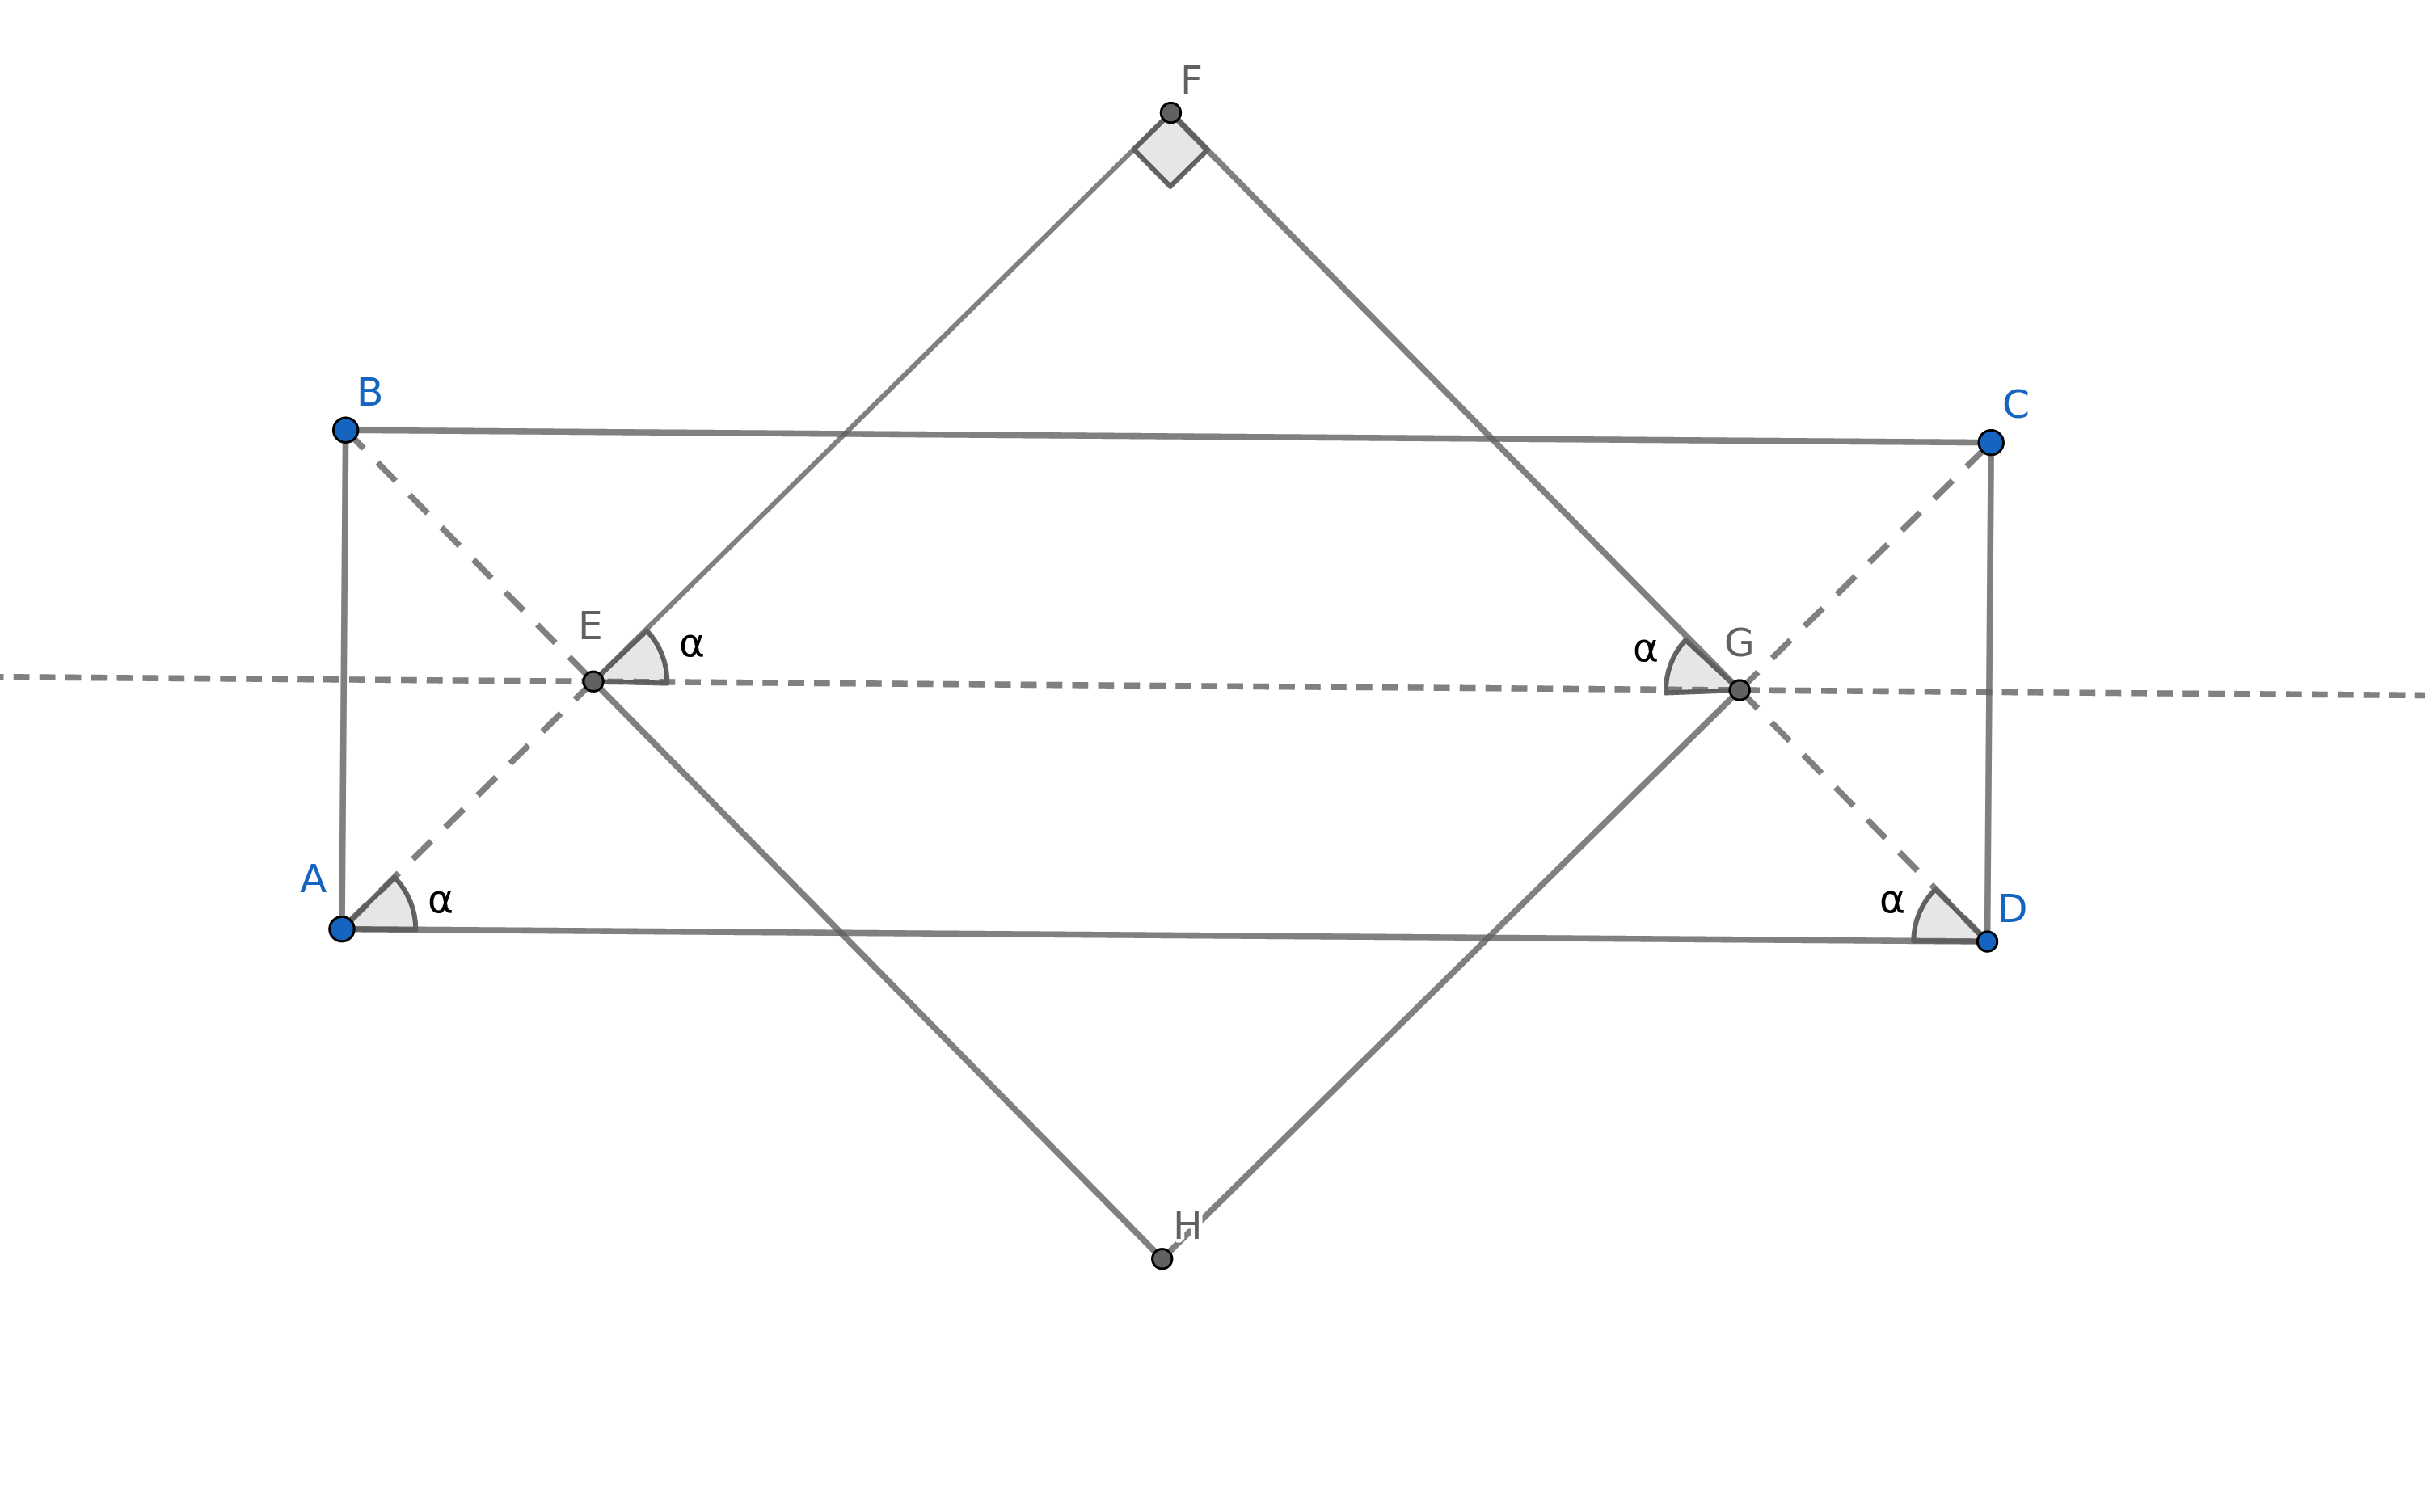
\includegraphics[width=1\linewidth]{pics/g2}
	\end{figure}
\end{sol}
\end{document}